\chapter{Fixing ADD\_ADDR}
\label{chap:addaddr2}

\section{The ADD\_ADDR2 format}
There is an ongoing effort to move the current MPTCP specification \ref{6824} from Experimental to Standard Track. Solving the ADD\_ADDR vulnerability is believed to be a fundamental step to reach the required security standards for the transition to happen.
By analyzing the nature of the vulnerability, various proposals have been elaborated to modify the design of the ADD\_ADDR option [\rfc{7430}]. The conceptual flaw behind the option is that no secret material related to the ongoing MPTCP is included. The only security mechanism connected to such message is indeed the TCP-level sequence and acknowledge numbers, that an attacker has to know in order to inject such message into an ongoing session.
A possible solution could be to add the receiver token of the connection as a field in the ADD\_ADDR option. Such token, exchanged only during connection establishment via the MP\_CAPABLE option, is supposed to be unknown to the attacker that in turns would not be able to forge a valid ADD\_ADDR message. This solution wouldn't be effective if the attacker is able to eavesdrop the keys during the initial handshake; keys' eavesdrop is indeed a security concern related to MPTCP [ref to section on Keys' Eavesdrop], and for this reason it is not advisable to add such information in clear inside the ADD\_ADDR option, since that would give more opportunities for eavesdropping.
Another possibility would be to maintain the ADD\_ADDR format unchanged but to block the attack at a later stage. For example, if the destination address of the SYN packet is added as part of the message used to calculate the HMAC value, the attacker wouldn't be able to recompute the HMAC value after modifying the destination address. However, since addresses are not a stable piece of information in a network with NATs, using the destination address to calculate the HMAC might not work.
In order to achieve higher security levels maintaining NAT compatibility, a third option has been proposed with positive feedback. The idea is to add to the ADD\_ADDR option a new field containing the truncated HMAC value (rightmost 64 bits) calculated as follow: the \textit{key} is the MPTCP key of the sender as originally agreed in the MP\_CAPABLE handshake; the \textit{message} is the concatenation of the previous three fields in packet: Address ID, advertised IP address, and Port. The new format (figure \ref{fig:addaddr2} has been formally specified for the first time in \rfc{6824bis-04}.

\begin{figure}[!htb]
\centering
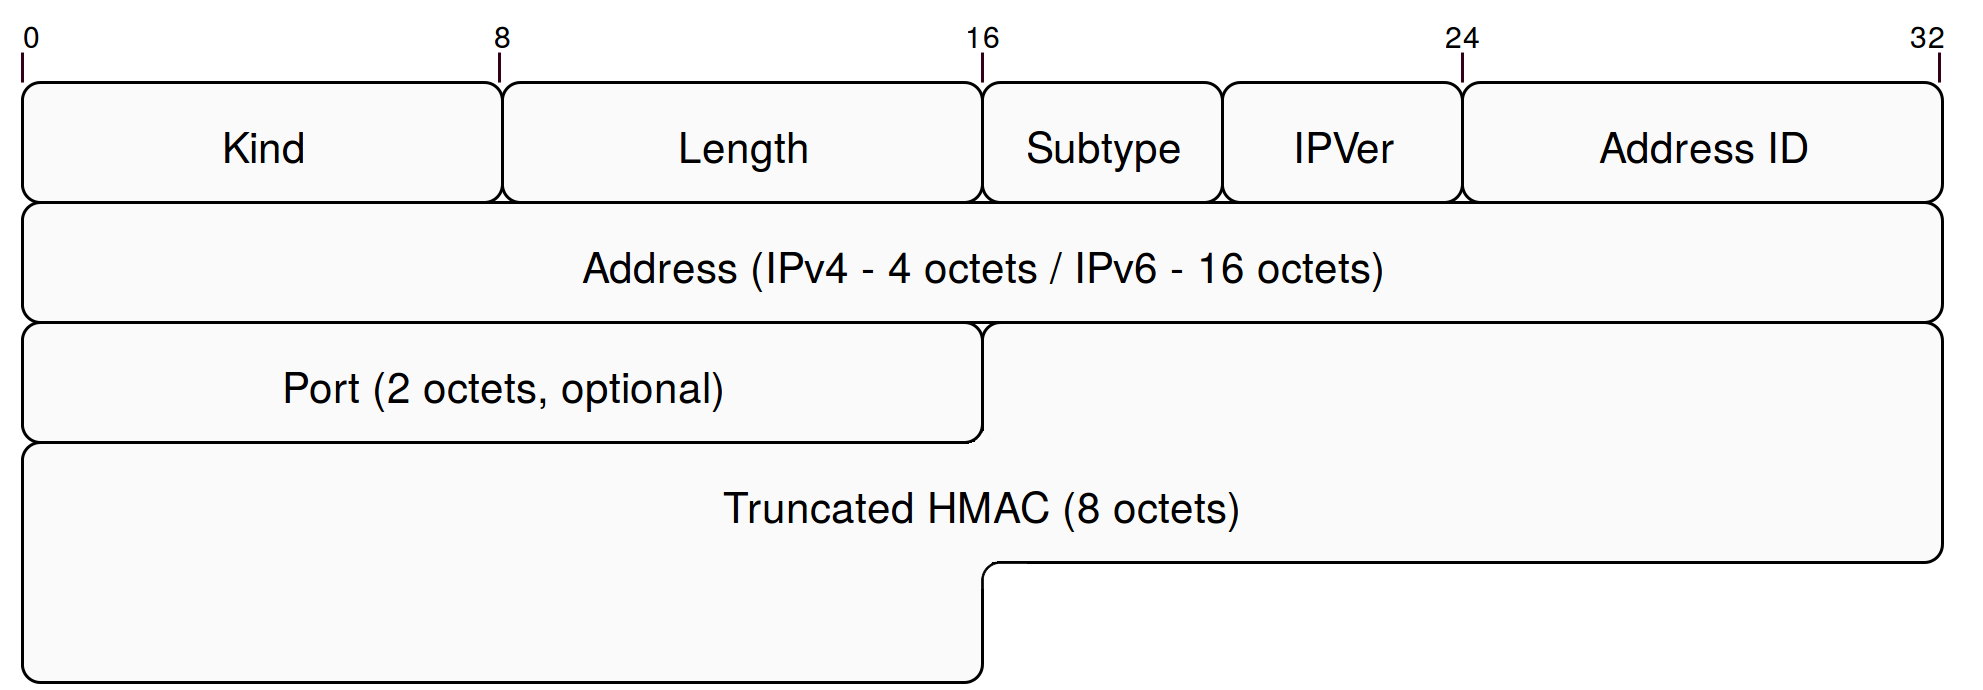
\includegraphics[width=0.75\textwidth]{images/addaddr2}
\caption{ADD\_ADDR2 option}
\label{fig:addaddr2}
\end{figure}

Such format would require the attacker to know the key in order to forge a valid ADD\_ADDR2 message, but such key is not exposed as in the case of the previous solution. Albeit, if the attacker is able to eavesdrop the keys during connection initiation it would be possible to exploit the same vulnerability even with the new address format. More experiments about this case are reported in section [ref to the experimental evaluation section]. Possible mitigations for such threat are explained in section [ref to keys' eavesdrop section 3.3.2].

The keys' eavesdrop threat is a partial-time on-path eavesdrop, a category that is considered less critical in terms of security concerns. Such keys' eavesdrop procedure in MPTCP has an almost identical counterpart in SCTP, when the SCTP-AUTH extension is used without pre-shared keys [\rfc{5061}]. In these regards the same security levels of SCTP would be reached in MPTCP by upgrading ADD\_ADDR to ADD\_ADDR2. Since SCTP is Standard Track, ADD\_ADDR2 is indeed considered a sufficient modification of the MPTCP first design to reach the security levels required for the transition to Standard Track.

\section{Implementing ADD\_ADDR2}
The current MPTCP patch added to the TCP stack in the Linux kernel currently counts around 12000 lines of code [\href{http://multipath-tcp.org/mptcp_stats/index.html}{href}]. It is considered the reference implementation for MPTCP and it closely follows RFC standards and set of features. Moreover, a lot of effort has been put into the implementation design in order to make the new protocol acceptable for upstream to the official Linux kernel. For such purpose, it is of paramount importance to keep the added complexity into the TCP stack as low as possible, in order not to jeopardize performance and stability of regular TCP. Nevertheless, high performance is expected for MPTCP. The main architectural concepts related to the control plane of the protocol are now explained, before introducing the modifications related to the new ADD\_ADDR2 format. 

\subsection{MPTCP in Linux}
With MPTCP in the Linux kernel, three main layers are introduced to guarantee multipath management and retro-compatibility with regular TCP [\href{http://inl.info.ucl.ac.be/publications/multipath-tcp-theory-practice}{href}]. The first element is the \textit{master subsocket}, which provides the interface used by the applications to communicate with the TCP stack. The structure of the master subsocket follows the regular TCP standards, in order to maintain retro-compatibility towards the application layer: in fact this is the only element used by the kernel in case of regular TCP connectivity. The second element is called \textit{multi-path control block (mpcb)} and it is the main brain of MPTCP, handling MPTCP-specific functionalities: the mpcb runs the algorithms that determine when to start or stop subflows, which subflow to chose in order to send a particular piece of data over the network and how to reconstruct the original data from the scattered segments coming from different subflows at the receiver. all the reordering algorithms in the mpcb work at the data-level, while the reordering of the data at the single subflows is handled by the underlying regular TCP. The final element of the MPTCP architecture is the set of \textit{slave subsockets}, the actual endpoints for the multiple MPTCP subflows. Such elements are not visible by the application, but they are handled by the mpcb. 
The master subsocket and the slave subsockets form the pool of subflows used in MPTCP.

% Change "multipath control block" with "meta-socket". mpcb is just a component of the meta-socket
\begin{figure}[!htb]
\centering
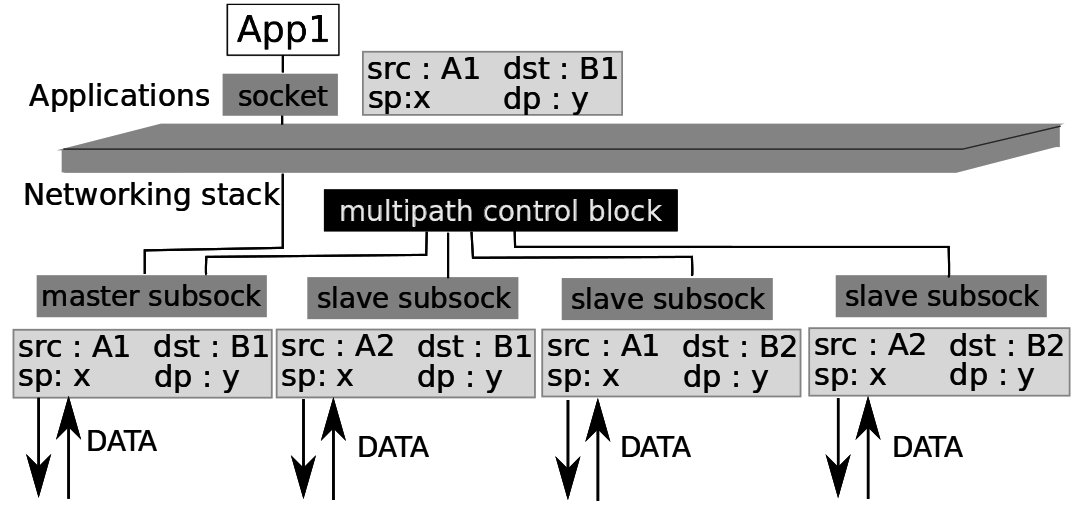
\includegraphics[width=0.75\textwidth]{images/architecture}
\caption{MPTCP Linux architecture}
\label{fig:architecture}
\end{figure}


Analyzing to the actual code implementation related to such architecture, it is mainly composed of several structures linked by pointers. In order to maintain the design-goal if minimizing the impact over regular TCP, when a TCP structure would need additional elements to handle MPTCP-related functionalities, the common choice is to define a new MPTCP-specific structure to store those elements. In this way, upon regular TCP operations, there would be no increase in memory-footprint and all the standard TCP structures would be in place. On top of that, having specific structures for MPTCP code makes it easier to read and understand the MPTCP parts inserted into the TCP stack. For example, a fundamental structure in TCP is the \textit{tcp\_sock} structure, that is used to store the state of a single TCP connection. In MPTCP, additional information for each TCP subflow is needed (for example the Address ID associated to each subflow). A new \textit{mptcp\_tcp\_sock} struct has been defined and each subflow contains a pointer to such new structure.
Also the previously mentioned main architectural element that is the multi-path control block is implemented in code using a new structure called \textit{mptcp\_cb}.

\begin{figure}[!htb]
\centering
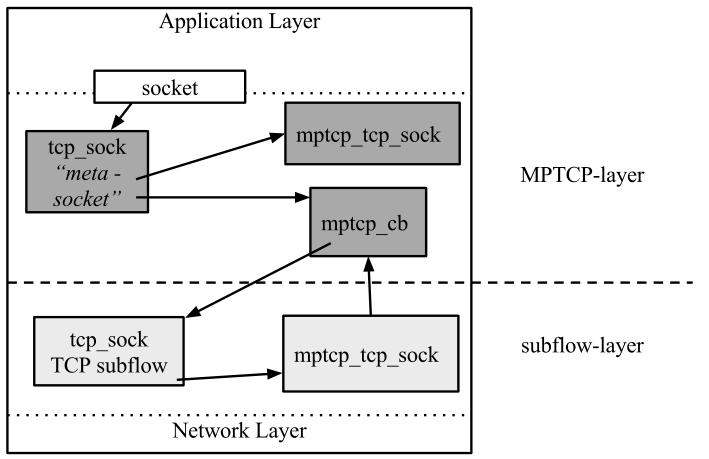
\includegraphics[width=0.7\textwidth]{images/structs}
\caption{MPTCP high-level data structures with relative references}
\label{fig:structs}
\end{figure}
%from Improving MPTCP

The allocation policy for all the new MPTCP structures is lazy-allocation, meaning that MPTCP structures are allocated only if it is detected that both hosts support the new protocol. This choice is again related to the main purpose of not affecting regular TCP when MPTCP fails during negotiation (or later on during the connection lifetime). A downside of this approach is related to the fact that the TCP stack operations are often executed in a soft-interrupt context, that does not allow functions to sleep in order to wait for available memory: this means that memory allocations might fail, forcing a fallback to regular TCP.
Nevertheless, connection setup in an MPTCP-compatible environment requires the client to send a first MP\_CAPABLE segment: this means that, even if no data structure is allocated during this first stage, the client has to generate a random key, and the related token is also calculated to check that it is not already used to identify another MPTCP connection. A reference to the originated \textit{tcp\_sock} structure is saved inside the hashtable used to keep track of the ongoing MPTCP connections. At this point, such \textit{tcp\_sock} is called "meta-socket". After that, if the SYN/ACK from the server does not contain a valid MP\_CAPABLE option, then the client simply removes the reference to the meta-socket from the hashtable before proceeding with a regular TCP handshake procedure. If the server side is MPTCP-compatible and the MP\_CAPABLE is indeed present in the incoming TCP segment, then the MPTCP structures are allocated: \textit{mptcp\_cb} and \textit{mptcp\_tcp\_sock}.
At the server, the status of the connection is not fully operational until the final ACK from the client as required by the TCP three-way handshake. When the SYN packet with MP\_CAPABLE option is processed, a \textit{request\_sock} data structure is allocated that has some additional space for MPTCP-related information with respect to the same structure used for regular TCP option. In case no MP\_CAPABLE option is present in the received SYN packet, the regular TCP version of the \textit{request\_sock} data structure is used, following the same design principles previously explained. The random key and uniqueness of the token are procedures executed at the server in a similar way with respect to the client. If all the MPTCP initialization procedure proceeds as expected, when the server receives the ACK from the client the master-socket is ready and linked to the \textit{mptcp\_cb}.
With the Linux kernel implementation of MPTCP, only the client is allowed to start the establishment of new subflows. There are two main reasons for this: if both client and server start a subflow at the same time, it can be that multiple path are established between the same pair of IP addresses, which can cause problems in some cases. Moreover, clients are often operating behind a NAT, which don't allow server to start new TCP sessions and consequently, they wouldn't allow the server to start a new subflow with the client.

After the connection has been established, multiple subflows can be used with MPTCP and there is a modular path-manager interface to allow flexibility in the heuristic adopted to decide which interfaces can be used and in which manner. In creating a new subflow, the client has to add the MP\_JOIN option inside the SYN packet and, differently from the MP\_CAPABLE scenario, the MPTCP-related structures like \textit{mptcp\_tcp\_sock} are created early on. At this point, failure wouldn't cause fallback to regular TCP and there is no need to risk memory allocation failures upon reception of the SYN/ACK from the server. Even if the subflows in MPTCP resemble regular TCP connections, the initial handshake differs in a way that it now requires four steps to reach fully operational status. The reason for this is that the third ACK now contains the HMAC value calculated by the client that has to be verified and acknowledged by the server before any data can be transmitted on such subflow. 
Regarding the operational flow in the stack upon reception of a SYN packet, there is no early inspection aimed at determining if an MP\_JOIN option is present: that would causes performance degradation in case of regular TCP SYN packets. Instead, the packet is processed with regular TCP stack until, in case of matching with a listening socket, the function \textit{tcp\_v4\_conn\_request()} is called: here the TCP options are scanned, and if MP\_JOIN is present then redirection to MPTCP happens, and the lookup in the hashtable is performed to determine which MPTCP connection the new SYN packet is addressing to. As a new addition required by MPTCP, if there is no matching socket found for the incoming packet, MPTCP still checks if the SYN message contains the MP\_JOIN option via the \textit{mptcp\_lookup\_join}. At this point, the server creates a request socket that is saved into the hashtable so that it can be retrieved when the client answers with the ACK message during the last stage of the subflow handshake.

This section presented an overview of the most important data structures and functions used in MPTCP to handle connection establishment and subflow management. The following sections will deal with the ADD\_ADDR functionality in the Linux kernel and how this was modified to implement the new format ADD\_ADDR2.



\subsection{Retro-compatibility}
Version control mechanism was not present but it is needed to negotiate which format to use in a MPTCP session: ADD\_ADDR or ADD\_ADDR2.

\subsection{Port advertisement}
Port advertisement in ADD\_ADDR is possible according to RFC specifications but it was not part of the implementation at the beginning of the thesis work, so it has been added.

\subsection{IPv6 considerations}
Longer addresses brought some issues related to TCP option fields limitations.

\subsection{Crypto-API in MPTCP}
A major problem was how to deal with the new hashing requirements introduced by ADD\_ADDR2. Extending the current MPTCP hashing function to deal with input messages of arbitrary size is a first point to explain. The second part has to deal with the whole analysis related to adopting the kernel CRYPTO APIs to calculate the HMAC values in MPTCP and why this is not advisable.

\section{Other contributions}
Another minor part of the thesis work on MPTCP is related to some small contributions to the official RFC documentation and other open-source projects.

\section{Experimental evaluation}
This part should include performance analysis regarding the new format introduced with ADD\_ADDR2. A discussion on how the new format (and all the other modifications introduced with the patches) could impact any aspect of the protocol should be present in this section.
It is possible to add here the other possible solutions for ADD\_ADDR fix, and why they are not good enough. 